\chapter{Memory organization and optimization}
\begin{flushright}
\english{Computer science has only three ideas: cache, hash, trash}\\ --- Greg Ganger, CMU
\end{flushright}
\minitoc

\section{Introduction}
\label{sec:associative-memory}

We need a way to organize the KB for efficient \textbf{information retrieval}.  This is critically important during inference and learning, where we need to pick some candidates for the next step of deduction or inductive learning, given the current \textbf{inference context}.

\section{Efficient rule fetching}

The current context is a set of propositions that are true currently.  Together with the goal which is the query (Let us focus on deduction for the time being;  the same technique that speeds up deduction will also speed up inductive learning).

An idea of Ben Goertzel's is that we can use \textbf{inference traces} to train a classifier to predict the best inference candidate.  A typical training example would be given as:\\
1. The goal (ie, the conclusion of a proof)\\
2. The context or premises (ie, facts residing in Working Memory)\\
Try to predict:\\
3. The next rule involved in the proof

So the function we need is:\\
\tab \{ fact \} $\times$ \{ set of facts \} $\mapsto$ rule

Using multidimensional scaling, we can map a fact to its coordinates in a high-dimensional space.

\section{Objective function}

Our objective is to reach the goal in a \textbf{proof tree}.  All the leaf nodes must be facts drawn from KB (red nodes), with some that are highlighted by the current context (purple nodes).  If we are backward chaining (BC), the goal is given.  If forward chaining (FC), we can find many goals and they can be scored by \textbf{interestingness}.
\begin{figure}[H]
\centering
\includegraphics[scale=1]{proof-tree.png}
\end{figure}

The difficulty of the rule recommendation problem is that at each iteration, we do not know the ultimate score of the conclusion(s) we may reach.  The situation may be similar to a chess game.  Factors affecting rule recommendation are:
\begin{compactenum-}
\item How likely is the rule to be satisfied given the current context (ie, the number of literals in the rule that remains to be satisfied)
\item Look-ahead to see what the rule can lead to, if satisfied;  This is also non-static, as it depends on the current inference context
\item How much interestingness the rule can contribute to the conclusion
\end{compactenum-}
Or, more precisely, we want to \textit{maximize expected interestingness}, given an inference context:
$$ \mathbb{E}[ \mbox{int} ] = \sum_{Cn \in {reachable \atop conclusions}} \mbox{int}(Cn) \cdot P(Cn | \mbox{ context, rule})  $$
The difficulty is in estimating $P(\mbox{reachable conclusions} | \mbox{ context, rule})$.  Notice that the reachable conclusions given a rule is relatively static;  what varies is the inference context (and to a lesser extent the facts in KB).  Indeed, given the context, we already have enough information to derive all possible conclusions.

\subsection{Interestingness}

The contribution to interestingness by a single rule can be measured by:
\begin{compactenum-}
\item How specific / general the rule is:  the most interesting rules select about half of its candidate objects;  A rule that is too general or too specific is not very useful
\item How high level the rule is -- a rule assigns conceptual labels to its objects, such concepts occupy certain places in the ontology
\end{compactenum-}

\section{Genetic / evolutionary methods}

We can construe this problem as a game:
\begin{compactenum-}
\item The moves are the selection of rules.
\item The score is given by the interestingness of final conclusion(s) and the time needed to arrive at them.
\item Perhaps we need some way to classify inference contexts and rules, to aid the selection of rules (ie, make the game easier to play).
\end{compactenum-}

The genetic algorithm needs to solve these:
\begin{compactenum-}
\item Organize contexts hierarchically
\item Organize KB hierarchically
\item Given context, fetch KB item, using the above hierarchies
\item Construct proof tree using unification
\end{compactenum-}

Alternatively we can partition the high-dimensional space into grids, and to each grid assign a bucket of rules.  We need some way to partition the high-dimensional space.  But we can also partition the space of data points into many categories?

\section{KB organization}

A new idea is to organize all rules in a \textbf{subsumption hierarchy}, and somehow filter the context through it.  The \textbf{Rules Tree} has at its root the most general rule (``everything is true'') and grows downward with successively more specialized rules.
\begin{figure}[H]
\centering
\includegraphics[scale=1]{rules-tree.png}
\end{figure}
  
In theory, we can embed the entire current state of the KB in the Rules Tree, by marking which conjuncts in the rules are satisfied by the current KB, but this may be impractical due to the large number of instantiations.  When we have a new inference context, we can traverse down the Rules Tree to the most specialized satisfiable rules, that will yield the most specialized derivable conclusions (from that rule).  Each of these conclusions will be fed through the Rules Tree again, recursively, until we reach enough interesting conclusions.  

The advantage of searching the Rules Tree is that we can terminate the search on a branch early on if the parent node is past its maximum truth value (thanks to subsumption ordering and peaking, see \S\ref{sec:subsumption-peaking}).

This technique should be augmented with rule indexing based on current context, so it can be quickly determined which rules are possibly unifiable with the context's proposition.

Or perhaps use a \textbf{stochastic local search} that begins in the middle of the Rules Tree.

But an interesting conclusion can be of high or low probability.

In the next iteration, we have the previous conclusion.  The new conclusion depends on that.  Perhaps we can back-track when stuck -- but how would back-tracking increase new conclusions?

In general, is it easier to satisfy general rules first?  Then we can successively refine the conclusions?  But that is not true if probability is the criterion.

\underconst

\subsubsection{The following is an older idea.}
\label{sec:hi-oracle}
What we need is in essence a \textbf{recommendation system}:  given an inference context, suggest a set of candidate rules.  An inference context is a set of (complete or partial) propositions.  The required mapping is \textbf{many-to-many}:  multiple propositions can recommend a rule, and a rule can be recommended by more than one proposition.
\begin{figure}[H]
\centering
\includegraphics[scale=1]{many-to-many-mapping.png}
\end{figure}

The KB is organized as an ontology (left), which we can abbreviate as a triangle (right).  Each logic formula can be classified into one of the ontology nodes (\textcolor{red}{red dots}).

A context is usually made up of several logic formulas (either complete or partial propositions;  \textcolor{Purple}{purple dots}).

The mapping we seek is:
\begin{figure}[H]
\centering
\includegraphics[scale=1]{ontology-triangular-form.png}
\end{figure}

Below is a detailed view of one possible scheme.  In this scheme, \textit{each proposition} in the context is mapped to a bag of rules.  Thus we ignore the \textit{combinatorial} effects of propositions in the context.  In this scheme, obviously, for each proposition we can recommend those rules that share at least one atom with the proposition -- because only those rules are unifiable with the proposition.  This is the maximum set of rules that are sensible to recommend, from which we can heuristically trim down.  Among these rules, only some would lead to our desired result.
\begin{figure}[H]
\centering
\includegraphics[scale=1]{rule-recommendation.png}
\end{figure}

The desired choice of rules will depend on the next inference steps which are opaque to us.  All we have are the clues from the current inference context (if forward-chaining), or additionally the goal (if backward-chaining).  

\underconst